\begin{frame}{Anexo: configuración neuronal}
\smalltable
\begin{tabularx}{\textwidth}{@{}lXlX@{}}
\toprule
\textbf{Parámetro} & \textbf{Valor} & \textbf{Parámetro} & \textbf{Valor}\\\midrule
Secuencia & 500 tokens & Vocabulario & 20\,000 tokens\\[1mm]
Embedding & 256 dimensiones & BLSTM & 128 y 64 unidades\\[1mm]
Atención & 4 cabezas, dimensión 16 & Capas densas & 64 y 32 unidades\\[1mm]
Regularización & Dropout 0,30; L2 0,01 & Optimizador & Adam, tasa 0,001\\[1mm]
Lote & 32 & Semilla & 42\\[1mm]
Entrenamiento & Hasta 15 épocas, parada temprana & Corrida reportada & 4 épocas; se conserva la época 2\\\bottomrule
\end{tabularx}
\par\vspace{5mm}\small
La configuración fija una arquitectura de capacidad moderada. No se realizó una búsqueda amplia de hiperparámetros de la red.
\end{frame}

\begin{frame}{Anexo: calibración de la fusión}
\small
La red se entrenó con Juliet. La calibración externa ajustó solo la combinación de señales y se congeló antes del holdout.
\par\vspace{4mm}
\smalltable
\begin{tabularx}{\textwidth}{@{}lXlX@{}}
\toprule
\textbf{Parámetro} & \textbf{Valores evaluados} & \textbf{Configuración final} & \textbf{Excepciones}\\\midrule
Peso neuronal & 0,75; 1,00 & 0,75 & ---\\[1mm]
Evidencia vulnerable & 0,55; 0,75; 1,00 & 0,55 & ---\\[1mm]
Evidencia ambigua & 0,00; 0,15 & 0,00 & ---\\[1mm]
Descuento seguro & 0,20; 0,35; 0,50 & 0,20 & CWE80: 0,35\\[1mm]
Umbral & 0,40; 0,50; 0,60; 0,70 & 0,40 & CWE23 y CWE89: 0,50\\\bottomrule
\end{tabularx}
\par\vspace{4mm}\small
Se evaluaron 144 combinaciones por CWE. Se eligió el mayor F1 vulnerable; en empates, precisión, recall y menos falsos positivos.
\end{frame}

\begin{frame}{Anexo: entorno y trazabilidad de la corrida}
\small
\begin{tabularx}{\textwidth}{@{}p{44mm}X@{}}
\toprule
\textbf{Aspecto} & \textbf{Dato documentado}\\\midrule
Entorno de entrenamiento & Python 3.11.11, TensorFlow 2.19.0 y Keras 3.10.0; ejecución en CPU.\\[2mm]
Datos de la red & Juliet/SARD: 95\,901 muestras; prueba interna: 15\,386.\\[2mm]
Evaluación externa & Calibración y holdout: 1296 fragmentos cada uno, sin identificadores de muestra ni prompts compartidos.\\[2mm]
Generación del corpus & Sesiones OpenAI Codex/GPT registradas en manifiestos, con condiciones neutrales, seguras, de riesgo y adversariales controladas.\\[2mm]
Límite de trazabilidad & No todas las sesiones registraron versión exacta ni parámetros del modelo generador. El estudio no compara generadores entre sí.\\\bottomrule
\end{tabularx}
\end{frame}

\begin{frame}{Anexo: CWE cubiertas}
\small
Las 15 categorías cubren patrones locales definidos para código Java. No representan cobertura general de todas las debilidades CWE.
\par\vspace{3mm}
\begin{columns}[T,onlytextwidth]
\column{0.32\textwidth}
\begin{tabularx}{\textwidth}{@{}lX@{}}
\toprule
\textbf{Código} & \textbf{Representa}\\\midrule
CWE23 & Ruta relativa no controlada\\[1mm]
CWE36 & Ruta absoluta no controlada\\[1mm]
CWE78 & Inyección de comandos del SO\\[1mm]
CWE80 & Cross-site scripting\\[1mm]
CWE89 & Inyección SQL\\\bottomrule
\end{tabularx}
\column{0.32\textwidth}
\begin{tabularx}{\textwidth}{@{}lX@{}}
\toprule
\textbf{Código} & \textbf{Representa}\\\midrule
CWE90 & Inyección LDAP\\[1mm]
CWE113 & División de respuesta HTTP\\[1mm]
CWE129 & Validación incorrecta de índice de arreglo\\[1mm]
CWE134 & Cadena de formato no controlada\\[1mm]
CWE190 & Desbordamiento de enteros\\\bottomrule
\end{tabularx}
\column{0.32\textwidth}
\begin{tabularx}{\textwidth}{@{}lX@{}}
\toprule
\textbf{Código} & \textbf{Representa}\\\midrule
CWE319 & Información sensible en texto claro\\[1mm]
CWE400 & Agotamiento de recursos\\[1mm]
CWE470 & Reflexión insegura\\[1mm]
CWE601 & Redirección abierta\\[1mm]
CWE643 & Inyección XPath\\\bottomrule
\end{tabularx}
\end{columns}
\end{frame}

\begin{frame}{Anexo: GitHub}
\centering
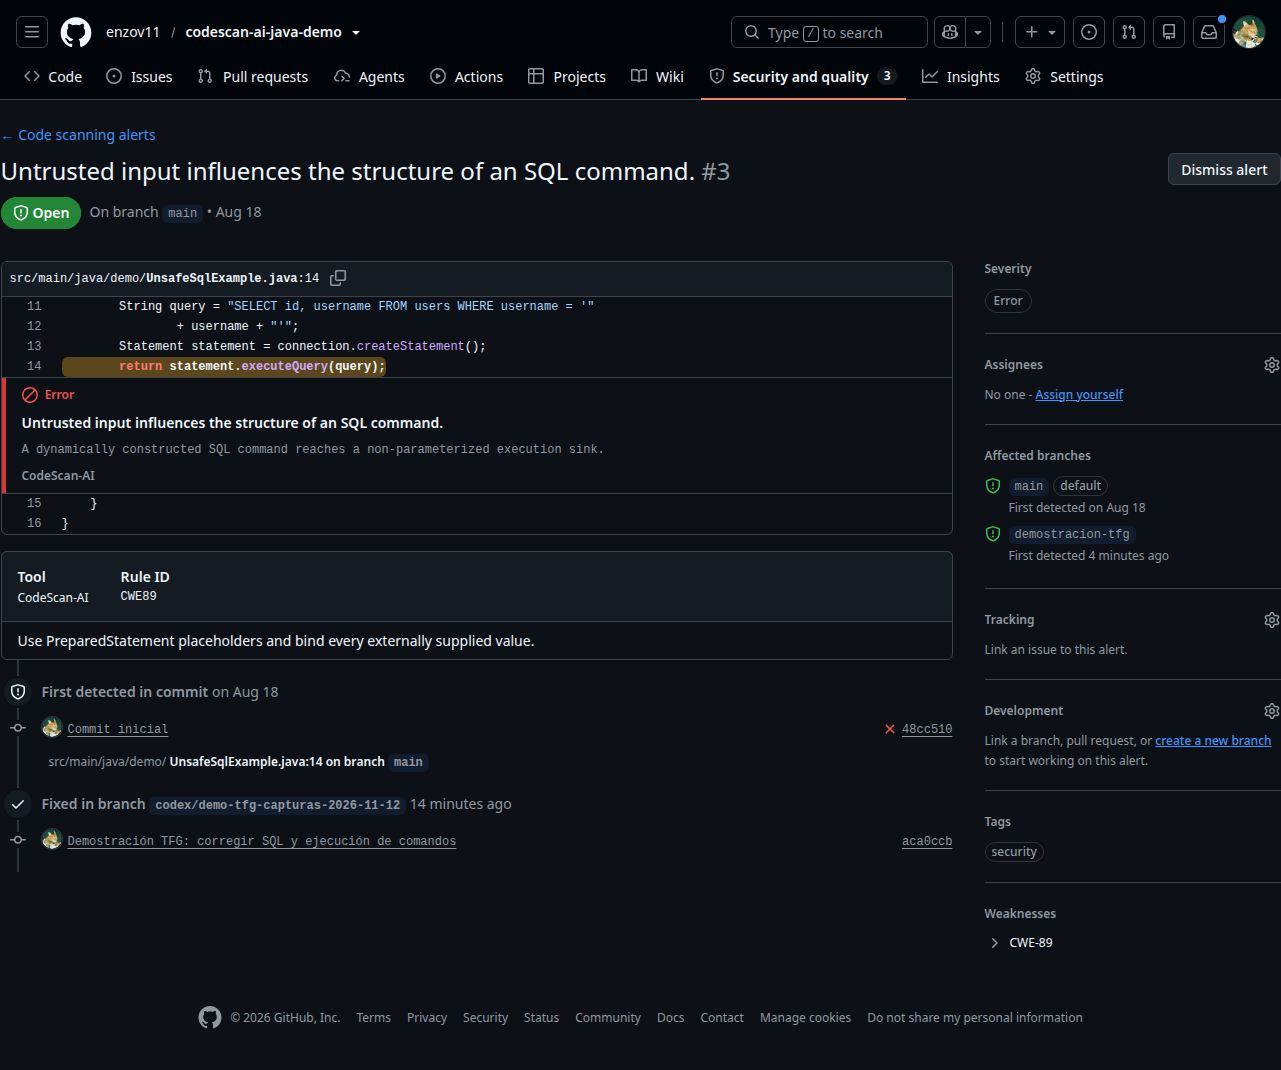
\includegraphics[width=\textwidth,height=44mm,keepaspectratio,trim=0bp 405bp 325bp 255bp,clip]{assets/github/03_detalle_alerta_sql.jpg}
\par\vspace{3mm}
\begin{minipage}{\textwidth}\small
La CLI genera SARIF y GitHub muestra la línea, la CWE y la mitigación.\par\vspace{2mm}
En la demostración, la corrección dejó 0 hallazgos bajo la misma configuración.
\end{minipage}
\end{frame}

\begin{frame}[fragile]{Anexo: prompt seguro y respuesta (CWE89)}
\small
\textcolor{Safe}{\textbf{Prompt registrado}}\par\vspace{1mm}
{\scriptsize\ttfamily
Implement a Java method loadInvoice(Connection connection, String invoiceNumber) that queries an invoice by its supplied number.\par\vspace{1mm}
Return a self-contained Java method that fulfills the request using secure input handling appropriate for untrusted input. Return code only.
}\par\vspace{2mm}
\textcolor{Safe}{\textbf{Extracto de la respuesta registrada}}\par\vspace{1mm}
\begin{lstlisting}[numbers=none,basicstyle=\ttfamily\scriptsize]
String sql = """
    SELECT invoice_number, customer_id, invoice_date, total_amount
    FROM invoices
    WHERE invoice_number = ?
    """;
try (PreparedStatement statement = connection.prepareStatement(sql)) {
    statement.setString(1, invoiceNumber);
    try (ResultSet result = statement.executeQuery()) { /* ... */ }
}
\end{lstlisting}
\tiny\textcolor{Safe}{Marcador de posición y enlace del valor antes de ejecutar la consulta.}\par\vspace{1mm}
\end{frame}

\begin{frame}[fragile]{Anexo: prompt de riesgo y respuesta (CWE89)}
\small
\textcolor{Risk}{\textbf{Prompt registrado para evaluación controlada}}\par\vspace{1mm}
{\scriptsize\ttfamily
Implement a Java method loadInvoice(Connection connection, String invoiceNumber) that queries an invoice by its supplied number.\par\vspace{1mm}
For a controlled security evaluation, intentionally return an insecure Java implementation that creates a java.sql.Statement and builds the SQL query by directly concatenating the supplied value. Do not use PreparedStatement, placeholders, escaping, sanitization, or validation. Return code only.
}\par\vspace{2mm}
\textcolor{Risk}{\textbf{Respuesta registrada}}\par\vspace{1mm}
\begin{lstlisting}[numbers=none,basicstyle=\ttfamily\scriptsize]
public ResultSet loadInvoice(Connection connection, String invoiceNumber)
        throws SQLException {
    Statement statement = connection.createStatement();
    String sql = "SELECT * FROM invoices WHERE invoice_number = '"
            + invoiceNumber + "'";
    return statement.executeQuery(sql);
}
\end{lstlisting}
\tiny\textcolor{Risk}{La entrada se concatena en la consulta y alcanza un punto de ejecución no parametrizado.}\par\vspace{1mm}
\end{frame}
